\documentclass[12pt,letterpaper,noanswers]{exam}
\usepackage[usenames,dvipsnames,svgnames,table]{xcolor}
\usepackage[margin=0.9in]{geometry}
\renewcommand{\familydefault}{\sfdefault}
\usepackage{multicol}
\pagestyle{head}
\definecolor{c03}{HTML}{FFDDDD}
\header{AM 22b Class 06}{Updated \today.}{Feb 8: Skill Check}
\runningheadrule
\headrule
\usepackage{graphicx} % more modern
\usepackage{amsmath} 
\usepackage{amssymb} 
\usepackage{hyperref}
\usepackage{tcolorbox}


\newcommand{\mb}[1]{\underline{#1}}

\begin{document}
 \pdfpageheight 11in 
  \pdfpagewidth 8.5in

% Name: \rule{2.5in}{0.5pt}
% \vspace{4mm}


\begin{questions}
\item Rewrite the equation of the plane
\[2x + y - z = 4 \]
\begin{itemize}
    \item in intercept form.
    \item using a dot product between a normal vector and a vector in the plane.
\end{itemize}

\vfill

\item \begin{parts}
\item Let $\mb{u}$ be the vector 
\includegraphics[scale=0.5]{img/C06p2a.png} and $\mb{v}$ be the vector 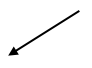
\includegraphics[scale=0.5]{img/C06p2b.png}.

Is $\mb{u}\times\mb{v}$ into the page/screen or out of the page (towards you)?

\vspace{1in}

\begin{oneparcheckboxes}
\choice into the page
\choice out of the page
\end{oneparcheckboxes}

\item Compute $(-\mb{i}+2\mb{j})\times(-2\mb{i}-\mb{j})$
\textbf{using distributive and scalar multiplication properties} of the cross product along with the cross product relationships between $\mb{i},\mb{j},\mb{k}$.

\framebox(250,50){ cross product:\hfill }
\vspace{1.5in}
\end{parts}
\end{questions}

\end{document}